\PassOptionsToPackage{dvipsnames}{xcolor}
\documentclass[border=0mm]{standalone}
\usepackage[dvipsnames]{xcolor}
\usepackage{amsmath}
\usepackage{amssymb}
\usepackage{dsfont}
\usepackage{bm}
\usepackage{tikz}
\usetikzlibrary{arrows}
\usetikzlibrary{calc}
\usetikzlibrary{shapes}
\usepackage{upgreek}

\usepackage{esvect}
\newcommand{\cev}[1]{\reflectbox{\ensuremath{\vv{\reflectbox{\ensuremath{#1}}}}}}


\definecolor{color1}{rgb}{0,0.4470,0.7410}
\definecolor{color2}{rgb}{0.8500,0.3250,0.0980}
\definecolor{color3}{rgb}{0.9290,0.6940,0.1250}
\definecolor{color4}{rgb}{0.4940,0.1840,0.5560}
\definecolor{color5}{rgb}{0.4660,0.6740,0.1880}
\definecolor{lightblue}{RGB}{86,192,150}

\pgfdeclarelayer{background layer}
\pgfdeclarelayer{foreground layer}
\pgfsetlayers{background layer,main,foreground layer}


\begin{document}



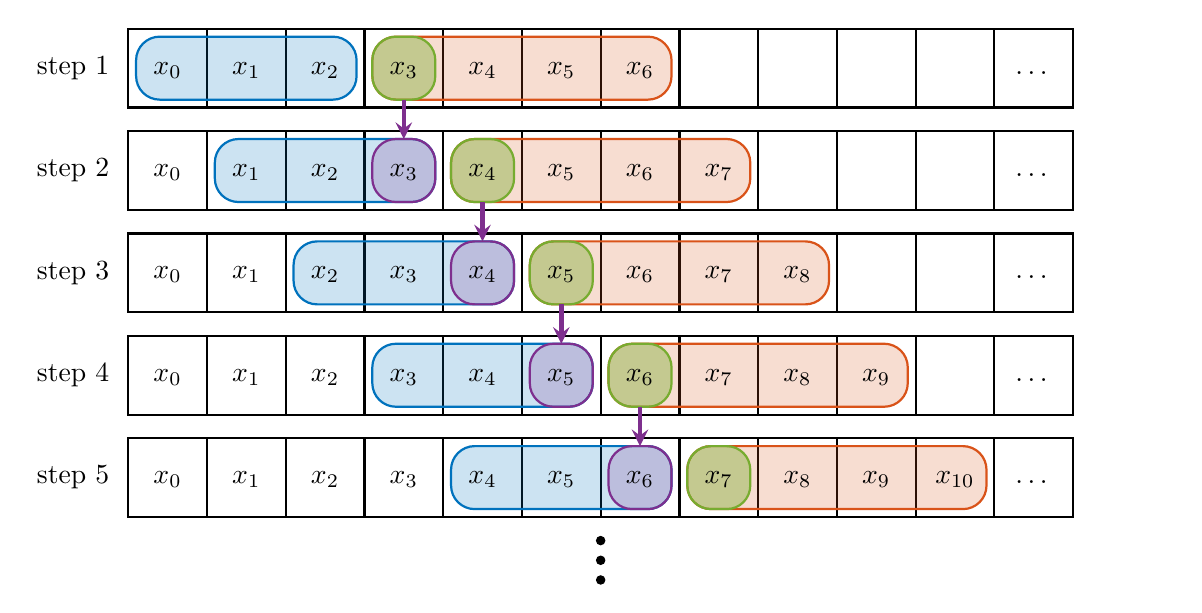
\begin{tikzpicture}[>=stealth,thick]

  \foreach \y in {1,...,5}{ 
    \foreach \x in {0,...,11}
    {    
     \draw [thick] (\x,-\y-0.3*\y) +(-.5,-.5) rectangle ++(.5,.5);
     \begin{pgfonlayer}{foreground layer}
     \ifnum\x=11
      \draw (\x,-\y-0.3*\y) node [anchor=mid]{$\dotsc$};
      \else
      \ifnum\x<\the\numexpr\y+6\relax
       \draw (\x,-\y-0.3*\y) node [anchor=mid]{$x_{\x}$};
	\fi
	\fi
      \end{pgfonlayer}
    }
    \node [] at (-1.2,-\y-0.3*\y) {step \y};
    \node [] at (12.2,-\y-0.3*\y) {\phantom{step \y}};
    \draw [thick,rounded corners =0.3cm, color1, fill=color1,fill opacity=0.2](\y-1,-\y-0.3*\y) +(-.4,-.4) rectangle ++(2.4,.4);
    \draw [thick,rounded corners =0.3cm, color2, fill=color2,fill opacity=0.2](\y+2,-\y-0.3*\y) +(-.4,-.4) rectangle ++(3.4,.4);
    \draw [thick,rounded corners =0.3cm, color5, fill=color5,fill opacity=0.4](\y+2,-\y-0.3*\y) +(-.4,-.4) rectangle ++(.4,.4);
    \ifnum \y<5
    \begin{pgfonlayer}{foreground layer}
    \draw [->,ultra thick,color4] (\y+2,-\y-0.3*\y-0.4) -- (\y+2,-\y-0.3*\y-1.3+0.4);
    \draw [thick,rounded corners =0.3cm, color4, fill=color4,fill opacity=0.2](\y+2,-\y-0.3*\y-1.3) +(-.4,-.4) rectangle ++(.4,.4);
      \end{pgfonlayer}
      \fi
}
    \draw [fill] (5.5,-7.3) circle (1.5pt);
   \draw [fill] (5.5,-7.55) circle (1.5pt);
   \draw [fill] (5.5,-7.8) circle (1.5pt);




\end{tikzpicture}

\end{document}







%\ifnum\y=3
%      \draw (\x,-\y-0.3*\y) node [anchor=center]{$\cdot$};
%      \draw (\x,-\y-0.35*\y) node [anchor=center]{$\cdot$};
%      \draw (\x,-\y-0.25*\y) node [anchor=center]{$\cdot$};
%      \else
%     \ifnum\y=4
%      \draw (\x,-\y-0.3*\y) node [anchor=mid]{$x_{\x,n}$};
%      \else
%      \draw (\x,-\y-0.3*\y) node [anchor=mid]{$x_{\x,\y}$};
%       \fi
















